% put all Mike's macros in and begin document
\documentclass[pdftex]{article}
\usepackage[pdftex]{graphics}
\usepackage{subfigure}
\usepackage{hhline}
\usepackage[usenames,dvipsnames]{color}
\usepackage{colortbl}
\usepackage[screen,pdftex]{mcdlecture}
\newcommand{\bs}{\relax}
\newcommand{\es}{\newpage}
\fboxsep=.01\textwidth \fboxrule=1pt
\newsavebox{\savepar}
\newenvironment{boxit}{\begin{lrbox}{\savepar}
    \begin{minipage}[b]{0.975\textwidth}}
    {\end{minipage}\end{lrbox}\framebox{\usebox{\savepar}}}


%%%%%%%%%%%%%%%%%%%%%%%%%%%%%%%%%%%%%%%%%%%%%%%%%%%%%%%%%%
%% THE FOLLOWING ARE THINGS THAT WE MIGHT CHANGE FROM YEAR TO YEAR OR
%% VENUE TO VENUE
    \lhead{MCMC in Statistical Genetics}
%   \lfoot{Dr Eric C. Anderson and Dr Matthew Stephens}
%    \lfoot{Dr Eric C. Anderson and Dr Matthew Robinson}
    \lfoot{Dr Matthew Stephens and Dr Matthew Robinson}
%	\lfoot{Dr Eric C. Anderson and Dr John Novembre}
    \rfoot{UW - Summer Institute, July 2019}
%	 \rfoot{Edinburgh - European Institute, June 2012}
%\rfoot{Brazil - Summer Institute, February 2014}

% on this one, be sure to update the venue and the module number
%\newcommand{\coursetitlepage}{European Institute in Statistical Genetics
\newcommand{\coursetitlepage}{Summer Institute in Statistical Genetics
%\newcommand{\coursetitlepage}{Brazilian Edition of the Summer \\Institute in Statistical Genetics

Module 18:

MCMC for Genetics}

%% Then update the schedule.  Note that I have broken that
%% out into a separate file like: schedule_table_edinburgh2012.tex
%% which is input in Overview.tex

%% Then be sure to change any time-sensitive events in the 
%% probability discussion in Matthew's first lecture.

%% And also update "structure_fun" link to my wiki to the right
%% year and venue.
%%%%%%%%%%%%%%%%%%%%%%%%%%%%%%%%%%%%%%%%%%%%%%%%%%%%%%%%%%


\begin{document}

\DeclareGraphicsExtensions{.jpg,.pdf,.png}%



%% Eric added a few things:
% some commands that Eric made for making a title while starting
% a new lecture and for making titles of new slides.
\newcommand{\newlecture}[1]{\newpage\begin{center}\section*{#1}\end{center}}
\newcommand{\newslide}[1]{\newpage\subsection*{#1: \hfil}}
 \newcommand{\Exp}{\Bbb{E}}
 \newcommand{\Var}{{\mathrm{Var}}}
 %% Some pretty etc.'s, etc...
\newcommand{\cf}{{\em cf.}}
\newcommand{\eg}{{\em e.g.},}
\newcommand{\ie}{{\em i.e.},}
\newcommand{\etal}{{\em et al.}\ }
\newcommand{\etc}{{\em etc.}}

%% some handy things for making bold math
\def\bm#1{\mathpalette\bmstyle{#1}}
\def\bmstyle#1#2{\mbox{\boldmath$#1#2$}}
\newcommand{\thh}{^\mathrm{th}}
\newcommand{\bpi}{{\pi}}
\newcommand{\mP}{\mathbf{P}}

\rhead{Monte Carlo - \thepage}




% each \include command puts a new file in.

% to make typesetting faster while working on a single
% section, but still have the appropriate page numbering
% and references, use the \includeonly command



\newlecture{Monte Carlo \\ (No Markov Chains\ldots Yet)}
Goals of this lecture:
\begin{itemize}
\item Define the Monte Carlo method generally
\item Explain why Monte Carlo is useful
\item Understand variance of Monte Carlo estimators
\end{itemize}
all without talking about Markov chains\ldots

%\newslide{The origin of Monte Carlo}
%
%First Reference:
%
%\textsc{Metropolis, N. and S. Ulam.}  1949.  The Monte Carlo method.  {\em Journal of the American Statistical Association}. 44:335--341.
%
%The name ``Monte Carlo" was coined originally by John von Neumann and Stanislaw Ulam who used the phrase as a code word at Los Alamos for their simulation-based computational methods used to solve the problem of initiating fusion in a thermonuclear bomb. 
%
%Earlier examples exist.  (for example, the Comte de Buffon and his needle in the mid-1700's).  
%
%With computer power increasing all the time, Monte Carlo methods are more widespread than ever, and are used in a wide range of applications, most of them of a more humanitarian bent than bomb design.    

\newpage

\includegraphics[width=\textwidth]{illus/JASA_MC_Article_Adding_Machine.pdf}
 

%\newslide{In search of a definition for Monte Carlo}
%There are few concise, yet general definitions in the literature.  Some, like Ripley (1987) reserve ``Monte Carlo" only for ``Monte Carlo Integration" and ``Monte Carlo Tests," and refer to all else as ``stochastic simulation."
%
%Others use Monte Carlo to refer specifically to the generation of pseudo-random numbers:
%   
%\begin{minipage}{.60\textwidth }
%{\sl ``One way to increase our confidence in the methods we use is to test models and methods on sets of data in which we know exactly what is happening\ldots A useful method for generating such data is called the Monte Carlo method.\ldots The Monte Carlo method uses random number generators for the construction of data."}
%\end{minipage}
%\hfill
%\begin{minipage}{.35\textwidth }
%\includegraphics[width=\textwidth]{illus/ecodetect}
%\end{minipage}


\newslide{A general definition of the Monte Carlo method}
\textsc{definition}: {\sl Monte Carlo is the art of approximating an expectation by the sample mean of a function of simulated random variables.}

This definition is general enough to encompass everything that has been called ``Monte Carlo," yet also makes clear its essence in familiar terms: Monte Carlo is about invoking laws of large numbers to approximate expectations.

\textsc{review:} {\sl Expectations}.
\[
\Exp[g(X)]= \int_{x\in\mathcal{X}} g(x)p(x)dx~~~~~~~~
\mathrm{or}~~~~~~~
\Exp[g(X)] = \sum_{x\in\mathcal{X}} g(x)p(x)
\]


\newslide{Breaking this down with a discrete example}

\vspace*{-1.3em}

\enlargethispage*{1000pt}
Imagine an organism with a distribution of family sizes (i.e., number of offspring), $s$:

\begin{minipage}{0.3\textwidth}
\begin{tabular}{ll}
$s$ & $p(s)$  \\ \hline
0 & 0.0184 \\
1 & 0.0735 \\
2 & 0.1469 \\
3 & 0.1959 \\
4 & 0.1959 \\
5 & 0.1567 \\
6 & 0.1045 \\ 
7 & 0.0597 \\
8 & 0.0299 \\
9 & 0.0133 \\
10 & 0.0053
\end{tabular}
\end{minipage}
~~
\begin{minipage}{0.68\textwidth}
The expected family size is:
$$
\Exp[S] = \sum_{s = 0}^{10} s p(s).
$$
But, perhaps you are interested in the expected number of
sibling pairs in a family.  If there are $s$ offspring, there are
$g(s) = s (s - 1) / 2$ sibling pairs in it.
$$
\Exp[g(S)] = \sum_{s = 0}^{10} [s(s-1)/2] p(s).
$$
\end{minipage}

\hrule
Important: For every Monte Carlo approximation there is an underlying expectation and a $g(x)$.  Get in the habit of identifying those.

\newslide{Laws of large numbers:}

\textsc{review:} {\sl Weak Law of Large Numbers}.\\
Let $X_1,X_2,\ldots,X_n$ be iid  r.v.'s with $\Exp|X_i|<\infty$, and $\bar{X}_n = \frac{1}{n}\sum_{1}^nX_i$.  Then 
\[
\lim_{n\rightarrow\infty} P(|\bar{X}_n - \Exp X_i| > \epsilon) = 0~~~~\mathrm{for~any}~\epsilon>0 
\]

Basically: if you take a sample mean of random variables, as your sample size gets very large, the sample mean gets very close to the expectation. 

This suggests: an expectation might be approximated by the sample mean of $n$ random variables (and it will work better if $n$ is large).
\[
	\Exp[g(X)] \approx \frac{1}{n}\sum_{i=1}^n g(x^{(i)})~~~~\mathrm{with}~~~X^{(i)}\sim p(x)
\]



\newslide{Why estimating expectations is useful}
Usually, any quantity of interest may be expressed as the expected value of a function of some random variable.  Importantly:
\begin{description}
\item[Probabilities:] 
\[
	P(X\in \mathcal{A}) = \Exp[ I_{\{\mathcal{A}\}}(X)]
\]
where $I_{\{\mathcal{A}\}}(X)$ is the {\em indicator function} taking the value 1 when $X\in\mathcal{A}$ and 0 otherwise.
\item[Integrals:] For a simple example, let $U$ be a uniform r.v. on the interval $[a,b)$ with pdf $p(u) = 1/(b-a)$.  Hence 
\[
	\int_a^b q(x)dx = (b-a)\int_a^b q(x)\frac{1}{b-a}dx = (b-a)\Exp[q(U)]
\]
We see here a case where Monte Carlo applies to a purely deterministic problem.
\item[Discrete Sums:] In the same vein as above, just as any integral can be approximated by Monte Carlo, so can any sum. For another simple, uniform example, let $W$ be a discrete random variable that takes all values $w$ in the set $\mathcal{A}$ with equal probability $P$. Then, the sum $\sum_{w\in\mathcal{A}}q(w)$ is easily approximated by Monte Carlo:
\[
	\sum_{w\in\mathcal{A}}q(w)  = {\displaystyle\frac{1}{P}  }
	\sum_{w\in\mathcal{A}}q(w)P = 
	{\displaystyle\frac{1}{P}  }
	\Exp[q(W)].
\]   
This is particularly useful in statistical genetics, because many probabilities of interest may be expressed as an intractable sum over latent variables.
\end{description}

The bottom line is that, since you can cast any quantity as an expectation; you can (in theory) approximate any quantity by Monte Carlo.  In the simplest case, when $X$ is distributed according to $p(x)$.  
\[
	\Exp[g(X)] \approx \frac{1}{n}\sum_{i=1}^n g(x^{(i)})~~~~\mathrm{with}~~~X^{(i)}\sim p(x)
\]

\newslide{Genetics example I: Estimating probabilities in the Wright-Fisher model}
The Wright-Fisher model underlies most population genetics theory that deals with the descent of genes in a finite population from one generation to the next.

A schematic of its underlying assumptions:
\begin{center}
\includegraphics[width=.52\textwidth]{illus/wfmodel.pdf}
\end{center}

\newslide{Genetics example I: Estimating probabilities in the Wright-Fisher model}
Let $X$ be the frequency of the $A$ allele in a Wright-Fisher population of size $N=100$ after 10 generations of drift, having started from a frequency of 30 out of 100.

\enlargethispage*{1000pt}
The distribution of $X$ can be approximated by simulating $n=10,000$ instances:
\begin{center}
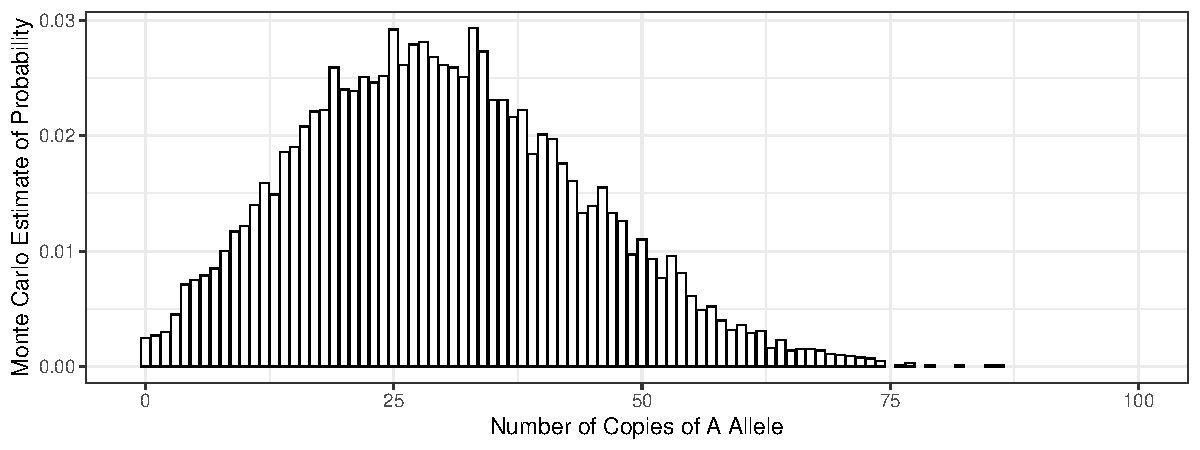
\includegraphics[width=0.9\textwidth]{figures/wf-100-by-10.pdf}
\end{center} 
\newpage
Each histogram column is an approximation of an expectation:
\begin{eqnarray}
		P(X = a) & = & \Exp[I_{\{x=a\}}(X)] \nonumber  \\
		&\approx & \displaystyle \frac{1}{n}
		\sum_{i=1}^n I_{\{x=a\}}(x^{(i)}) \nonumber
\end{eqnarray}
for $a=0,1,\ldots,100$, where each $x^{(i)}$ is an independent realization of the 
number of $A$ alleles at $t=10$ in the Wright-Fisher model.
\newslide{Genetics example II: estimating a sum over latent variables} Wright and McPhee (1925) estimating inbreeding of individuals within cattle pedigrees.
\begin{center}
\includegraphics[width=.83\textwidth]{illus/cows.pdf}
\end{center}
In terms of latent variables:
\begin{itemize}
\item The maternal ($m$) and paternal ($p$) genes in individual $z$ are direct descendants from an {\em unobserved} lineages of ancestral gene copies, $A_m$ and $A_p$ from $z$ up to a founder in the pedigree.
\item The individual is inbred at a locus if the ancestors of the maternal gene and the paternal gene are the same at any point in their lineages, \ie ~if the lineages $A_m$ and $A_p$ hit one another going back up the pedigree.
\item The probability that an individual is inbred at a locus is then the sum over latent variables:
\[
	P(\mathrm{inbred}|\mathrm{pedigree}) = \sum_{A_m,A_p} [I_{\{A_m~\mathrm{``hits"}~A_p\}}(A_m, A_p )] P(A_m,A_p)
\]
where $P(A_m,A_p)$ follows from Mendel's laws.  Note that $A_m$ and $A_p$ are independent up until they intersect, then follow the same lineage back in time.
\newpage
\item This sum is an expectation of the indicator function, with respect to the joint distribution of $A_m$ and $A_p$, given the pedigree:
\[
	P(\mathrm{inbred}|\mathrm{pedigree}) = \Exp [I_{\{A_m~\mathrm{``hits"}~A_p\}}] 
\]
so it may be estimated by Monte Carlo:
\begin{eqnarray}
	P(\mathrm{inbred}|\mathrm{pedigree}) & = & \Exp [I_{\{A_m~\mathrm{``hits"}~A_p\}}] \nonumber \\
& \approx &
\frac{1}{n}\sum_{i=1}^n I_{\{A_m~\mathrm{``hits"}~A_p\}} \nonumber
\end{eqnarray}
where $A_m^{(i)}$ and  $A_p^{(i)}$ are simulated from their respective distributions, which can be done by flipping a coin, until they intersect (and hence add 1 to the sum) or reach pedigree founders without intersecting (adding 0 to the sum).
\end{itemize}



\newslide{Sampling From Posterior Distributions}

\begin{itemize}
\item In Bayesian statistics, Monte Carlo sampling is often done from the
posterior distribution. 
\item Imagine a posterior distribution for $Q$ that is a $\mathrm{Beta}(30, 70)$
distribution.  
\item If you want to know the posterior probability that $Q > 0.35$ that probability is an expectation:
$$
P(Q > 0.35) = \Exp[I_{\{q > 0.35\}}(Q)]
$$
\item Here, $g(Q) = I_{\{q > 0.35\}}(Q)$, a function that returns a 1 if $Q > 0.35$ and a 0 otherwise. This expectation can be approximated by Monte Carlo with
$$
P(Q > 0.35) = \Exp[I_{\{q > 0.35\}}(Q)] \approx 
\frac{1}{n} \sum_{i=1}^n I_{\{q > 0.35\}}(q^{(i)})	
$$
\end{itemize}

\newslide{Variance of Monte Carlo estimators---iid case}
A Monte Carlo estimator is simply a random variable itself---a sum of random variables:
\[
	G_n = \frac{1}{n}\sum_{i=1}^n g(X^{(i)})
\]
So, if the $X_i$ are independent\footnote{Note that throughout most of the remainder of the course, we will deal with samples of correlated, non-independent $X_i$'s.  This is just a warm-up.} the variance of $G_n$ is easily computed as the variance of a sum of independent R.V.'s:
\begin{eqnarray}
	\Var(G_n) & = & \Var\biggl(\frac{1}{n}\sum_{i=1}^n g(X^{(i)})\biggr) = \frac{1}{n^2}\sum_{i=1}^n \Var[g(X^{(i)})] \nonumber \\
	&=& \frac{\Var[g(X^{(i)})]}{n} \nonumber
\end{eqnarray}
$\Var \downarrow$ when $n\uparrow$ or if $\Var[g(X^{(i)})]$ can be reduced\footnote{We'll take this up later in our discussion importance sampling}.




\end{document}


